\documentclass{standalone}
\usepackage{tikz}

\begin{document}

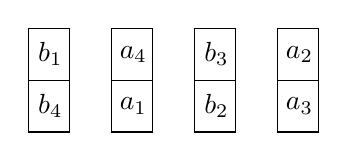
\begin{tikzpicture}[x=0.8pt,y=0.75pt,yscale=-1.25,xscale=1.25]
%	\useasboundingbox  (-5pt,-15pt) rectangle (85pt,31pt);
%cluster 1
\def\x{30}
\def\w{15}
%Shape: Rectangle
\draw   (0,0) -- (15,0) -- (15,40) -- (0,40) -- cycle ;
%Straight Lines
\draw   (0,20) -- (15,20) ;
% Text Node
\draw (8,10) node (b1)  {$b_{1}$} ;
% Text Node
\draw (8,30) node (b4)   {$b_{4}$};

%cluster 2
\draw   (\x,0) -- (\w+\x,0) -- (\w+\x,40) -- (\x,40) -- cycle ;
\draw   (\x,20) -- (\w+\x,20) ;
% Text Node
\draw (\x+8,10) node (a4)   {$a_{4}$};
% Text Node
\draw (\x+8,30) node (a1)   {$a_{1}$};

%cluster 3
\draw   (2*\x,0) -- (\w+2*\x,0) -- (\w+2*\x,40) -- (2*\x,40) -- cycle ;
\draw    (2*\x,20) -- (\w+2*\x,20) ;
% Text Node
\draw (2*\x+8,10) node (b3)   {$b_{3}$};
% Text Node
\draw (2*\x+8,30) node (b2)   {$b_{2}$};

%cluster 4
\draw   (3*\x,0) -- (\w+3*\x,0) -- (\w+3*\x,40) -- (3*\x,40) -- cycle ;
\draw    (3*\x,20) -- (\w+3*\x,20) ;
% Text Node
\draw (3*\x+8,10) node (a2)   {$a_{2}$};
% Text Node
\draw (3*\x+8,30) node (a3)   {$a_{3}$};
\end{tikzpicture}


\end{document}